\documentclass{TDP005-mall}
\usepackage{graphicx}
\graphicspath{ {images/} }


\newcommand{\version}{Version 0.2}
\author{Gustav P Svensson, \url{gussv375@liu.se}\\
  Love Bäckman, \url{lovba497@liu.se}}
\title{Designspecifikation}
\date{2016-11-25}
\rhead{Gustav P Svensson\\
Love Bäckman}



\begin{document}
\projectpage
\section{Revisionshistorik}
\begin{table}[!h]
\begin{tabularx}{\linewidth}{|l|X|l|}
\hline
Ver. & Revisionsbeskrivning & Datum \\\hline
0.1 & Påbörjat utkast & 161123 \\\hline
0.2 & Första utkast klart & 161125 \\\hline
\end{tabularx}
\end{table}


\section{UML - Klassdesign}
När spelet startas skapas en spelmotor som skapar två stadieobjekt, ett menystadie och ett spelstadie. Stadierna har en variabel <active> som håller reda på om stadiet är aktivt eller inte, per default är <active> true för menystadiet och false för spelstadiet.
\\\\
I spelmotorn körs spelloopen som anropar det aktiva stadiets körfunktion. Körfunktionen  hanterar händelser inuti spelstadiet och skickar tillbaka en vector med alla objekt i stadiet, vilka sedan renderas av spelmotorn. I slutet av varje loop kontrolleras om det aktiva stadiets <active> variabel fortfarande är true, om inte sätts det andra stadiets <active> variabel till true.
\\\\
När spelaren väljer en nivå i menystadiet kommer menystadiets <active> variabel sättas till false och den valda nivån objekt laddas in i spelstadiet, vars <active> variabel sätts till true.
\\\\
Om spelaren sedan återgår till menystadiet kommer spelstadiet att ligga intakt, vilket innebär att spelaren, om den vill, kan återgå till spelstadiet och fortsätta där den slutade istället för att läsa in en ny nivå.

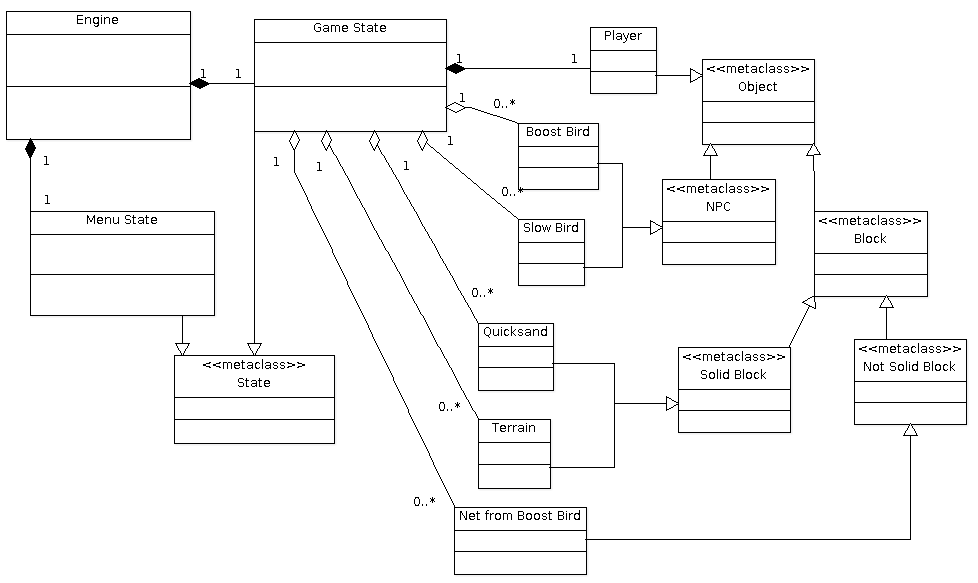
\includegraphics[scale=0.5]{ClassDiagram}

\end{document}
